% \chapter*{Additional Problems}

\begin{aproblem}{Graphing Motion I:  Bouncing Ball.}
  \begin{enumerate}
  \item Pick up your larger superball (the one in your toy kit with
    the bug or skull inside it), toss it straight up, and catch it
    when it comes back down to your hand.  Watch the motion very
    carefully.  Answer the following questions: Just after the ball
    leaves your hand, is the speed the largest, in the middle, the
    smallest, or zero? Is the velocity direction up or down?

    Answer the same questions for the ball when it is halfway up to
    its highest point, when it is at its highest point, when it is
    halfway down, and when it reaches your hand again.
 
  \item Now, make sketches of the ball's ({\it i}) vertical position versus
    time (choose ``up'' as the positive direction and $y = 0$ as the
    ground) as the ball rises and then falls back to your hand, ({\it ii})
    velocity versus time, and ({\it iii}) acceleration versus time.  Don't
    worry about putting any numbers on the graphs; just make a
    qualitative sketch.  {\bf Make sure that your plot of velocity
      versus time agrees with the answers from part~a).}

  \item Drop the ball on the ground and watch it carefully as it
    bounces up and down a few times.  Answer the following questions:
    {\em just before} the ball hits the ground, is the speed at its
    peak (i.e., large), in the middle, near its slowest value, or
    zero, and does the velocity point upward or downward?  Answer the
    same questions for the ball {\em just after} it hits the ground
    and starts moving upward.

  \item Now, make qualitative sketches of the ball's ({\it i}) vertical
    position versus time as the ball drops toward the ground before
    the bounce, and while the ball moves away from the ground after
    the bounce, ({\it ii}) velocity versus time, and ({\it iii}) acceleration
    versus time.  {\bf Make sure your plot of velocity agrees with the
      answers from part c).}

  \item Consider what the graphs of vertical position versus time,
    velocity versus time, and acceleration versus time look like for
    the short period of time while the ball is in contact with the
    ground.  Sketch on your graph from part d).
 
  \end{enumerate}
  \label{prob:bouncing_ball}
\end{aproblem}

\begin{aproblem}{Graphing Motion II: Spring and Return Ball.}
  \begin{enumerate}
  \item Take your round metal spring and your ``return ball'' (the
    little rubber ball attached to an elastic string).  The return
    ball is the perfect size to jam into one end of the metal spring,
    so do this.  Hold the spring from the other end, and let the
    spring/ball system hang vertically and allow it to come to rest
    (you are welcome to use your other hand to help the end of the
    spring with the ball stop moving).  Be careful that the string on
    the return ball doesn't get tangled in the spring.
 
  \item Call the position of the ball when it is motionless $y = 0$.
    Now, pull the ball end of the spring straight down approximately 6
    -- 10 inches (the exact distance isn't that important) and release
    the ball end of the spring.  Make sure that the subsequent motion
    of the ball and the spring is as vertical as possible.

  \item Make qualitative plots of the ball's ({\it i}) vertical position
    versus time for a few cycles, and ({\it ii}) vertical velocity versus
    time.  Use your sketch of the ball's vertical velocity versus time
    to make a qualitative sketch of the ball's vertical acceleration
    vs. time.  (Hint: ask the same questions as in Problem
    A\ref{prob:bouncing_ball} if you are stuck.  Specifically consider
    the ball's position and velocity when it is at the maximum
    distance from $y = 0$ and also consider the ball's position and
    velocity when it is passing through $y = 0$.)
  \end{enumerate}
  \label{prob:graphII}
\end{aproblem}


\begin{aproblem}{Falling Birdie.}  Consider a badminton birdie that is
  falling under the influence of gravity and air resistance.  Assume
  that the vertical acceleration of this birdie is given by
  \[ a_y = \frac{dv}{dt} = g - bv, \] 
  where $g = 9.8\units{m/s$^2$}$ and $b$ is some constant that
  depends on the mass and shape of the birdie along with properties of
  the air, and $v$ is the instantaneous velocity of the bird (positive
  if the velocity is down and negative if the velocity is up).
  Suppose that the birdie is released from rest at time $t=0$.

  \begin{enumerate}

  \item Discuss qualitatively how the speed of the birdie varies with
    time, given your knowledge of the relationship between the
    acceleration and the rate of change of the velocity.  What is the
    velocity when the acceleration is zero?  (This is called the
    terminal velocity.)  What happens to the velocity after the
    acceleration reaches zero?

  \item Without solving the equation above, sketch $v(t)$ vs. $t$.
    This can be done as follows: at $t=0$, $v$ is zero and the slope
    is $g$.  Sketch a straight-line segment, neglecting any change in
    the slope for a short time interval. At the end of the interval,
    the velocity is no longer zero, so the slope is no longer $g$.
    Sketch another straight-line segment with the qualitatively
    appropriate slope for the next short time interval.  Continue
    until your sketch shows the birdie has reached terminal velocity.
    What is the slope of the line after the birdie has reached
    terminal velocity?
  \end{enumerate}
  \label{prob:falling_birdie}
\end{aproblem}

\begin{aproblem}{Estimating Velocities: Muzzle Speed of a Blow Dart.}
  \label{prob:dartI}
  Be careful!  Students in the past have set off the sprinkler and
  fire alarms in their dorms!  Consider doing this outside or
  somewhere where the ceiling is very high.
  \begin{enumerate}
  \item To estimate the ``muzzle speed'' of a blow dart, fire the dart
    straight up into the air and time how long it takes to come back
    down.  Roughly half of that time is the time for the object to
    decelerate from its initial velocity to motionless (at the top of
    its motion).  {\bf Warning:} students often over-estimate the time
    required for the trip.  Remember to count ``0'' when you fire the
    dart (``0 and 1 and 2 and \dots'')

  \item Now, use
    \[ a_{\rm avg} = \frac{\Delta v}{\Delta t} \] to estimate the
    initial velocity.  {\bf Keep this estimate handy:} you'll use it
    later on in this unit.
  \end{enumerate}
\end{aproblem}


\begin{aproblem}{Graphing Motion III: Blow darts.}
  \begin{enumerate}
  \item Fire a blow dart roughly horizontally (don't worry about the
    vertical motion here) at a smooth surface on which it will
    stick. (Windows make nice targets, but be careful with flat panel
    displays --- students have broken them in the past with their blow
    darts!)

  \item Make qualitative plots of ({\it i}) the dart's horizontal position
    versus time up until and shortly after the dart hits its target,
    ({\it ii}) the dart's horizontal velocity; and ({\it iii}) the dart's
    horizontal acceleration.  In the plot of acceleration, include the
    small time interval between when the dart first makes contact to
    when it is completely compressed and stuck.  (Hint: ask the same
    questions as in Problem A\ref{prob:bouncing_ball} if you are
    stuck.)
  \end{enumerate}
\end{aproblem}

\begin{aproblem}{Rocket Motion.}
  A rocket lifting off from a launch pad in Florida has a vertical
  position given by
  \[ y(t) = 70 + 40t + 0.3t^3 \] during the first moments of takeoff,
  where $y$ is the height of the rocket in meters and $t$ is the time
  in seconds after the rocket clears the support tower.  Assuming the
  motion of the rocket is purely vertical, determine both the speed
  and the acceleration of the rocket at time $t = 10\units{s}$.
  \label{prob:rocket_motion}
\end{aproblem}



\begin{aproblem}{Average Velocity: Round Trip of a Blow Dart.}
  \begin{enumerate}
  \item Fire a blow dart straight up into the air and wait for it to
    come back down to its initial position.  {\bf Question:} for the
    entire flight, what is the average velocity?  (A very quick
    estimate is fine --- if this question takes you more than 1 or 2
    minutes to answer, then discuss this with a friend or your problem
    session instructor.)

  \item Now, fire the blow dart at an angle somewhere in the vicinity
    of $45^\circ$ (the actual angle isn't critical).  Watch the entire
    flight, and comment on the average velocity (both magnitude and
    direction --- if not zero).
  \end{enumerate}
  \label{prob:blow_dart}
\end{aproblem}



\begin{aproblem}{Vector Addition: Walking Around.}
  \begin{enumerate}
  \item Using the method of components, add the following vectors, and
    determine the $x$-component and $y$-component of the total, and
    the magnitude and direction of the total: 10 paces at $45^\circ$,
    12 paces at $90^\circ$, 17 paces at $-45^\circ$, and 10 paces at
    $-135^\circ$.

  \item {\bf Do the experiment.}  [We will do the following as a class
    exercise during problem session, so you don't have to do this on
    your own.]  On a sunny day, pick a starting location in the middle
    of an open field or grassy area. (Lamp posts work well.)  Choose
    the direction that your shadow casts as the $0^\circ$ direction
    and imagine a $360^\circ$ arc around that direction.  Now, walk 10
    paces at an angle of $45^\circ$ (you'll be taking your shadow with
    you, so you'll be able to see that you are walking at the correct
    angle).  Then, walk 12 paces at an angle of $90^\circ$, 17 paces
    at an angle of $-45^\circ$, and 10 paces at $-135^\circ$.  Where
    do you end up relative to your starting location?  Does this agree
    with your calculation?  Write down how you compared your result
    with your calculation.

  \item Now, do the same experiment again starting from the same
    initial location.  {\bf But this time} walk off the vectors in a
    very different order, say, 10 paces at an angle of $-135^\circ$,
    17 paces at an angle of $-45^\circ$, 12 paces at an angle of
    $90^\circ$, and 10 paces at an angle of $45^\circ$.  Do you end up
    in the same place as you did in the previous experiment?  (You
    should.)  Comment on your results.
  \end{enumerate}
\end{aproblem}

\begin{aproblem}{Hello Kitty.}  
  A kitten, who has been napping in a patch of sun, sees a flying bug
  and sprints $3\units{m}$ due North.  She leaps straight up in the
  air, misses the bug, and comes straight back down.  She then calmly
  strolls $5\units{m}$ in a direction $40^\circ$ S of W, where she
  spits up a hairball under the kitchen table, then walks $2\units{m}$
  in a direction $30^\circ$ S of E where she begins to lick up some
  spilled milk.
  \begin{enumerate}
  \item Draw a diagram showing all the displacements of the kitten.
  \item The kitten's sister was napping with the kitten in the patch
    of sun.  How far and in what direction should the kitten's sister
    walk to go directly from the patch of sun to the spilled milk?
  \end{enumerate}
\end{aproblem}



\begin{aproblem}{Love Boat.} 
  Juliet is traveling on a fast gondola that is moving at a constant
  speed of $10\units{m/s}$ down a canal.  Romeo is standing still on
  the bank of the canal and watching the gondola go by.  To attract
  his attention, Juliet throws her ring into the air and catches it as
  it falls.  Relative to the gondola, the initial velocity of the ring
  is $15\units{m/s}$ straight up.  Answer the following questions
  according to {\bf both} Juliet and Romeo.  Neglect the effects of
  air resistance in this problem.
  \begin{enumerate}
  \item What is the magnitude and direction of the initial velocity of
    the ring?
  \item How long is the ring in the air?
  \item What horizontal distance has the ring traveled?
  \item What is the minimum speed of the ring while it is in the air?
  \item What is the acceleration of the ring while it is in the air?
  \end{enumerate}
\end{aproblem}

\begin{aproblem}{Graphing Forces: The Large Superball.}
  \begin{enumerate}
  \item Continuing from Problem~A\ref{prob:bouncing_ball}: Toss your
    large superball straight up in the air and catch it when it comes
    back down.  Make a qualitative graph of {\em net force} acting on
    the ball versus time while in the air (you can neglect air
    resistance here).  Compare this graph with the ones that you made
    for Problem~A\ref{prob:bouncing_ball}.  What is the net force
    acting on the ball at the top of its motion (when it stops its
    upward motion and starts falling back down)?  How does the force
    at the top of its motion relate to the acceleration (from
    Problem~A\ref{prob:bouncing_ball})?

  \item Now, make a graph of net force acting on the ball versus time
    {\em including} the effects of air resistance on the ball.  In
    doing this, you'll need to think about the direction of the
    resistive force, as well as how its magnitude depends on its
    motion.
  \end{enumerate}
\end{aproblem}

\begin{aproblem}{Tension: Playing with the Return Ball.}
  \begin{enumerate}
  \item Take the ``return ball'' (the little rubber ball attached to
    an elastic string) and hang it straight down.  Wait for it to stop
    moving.  Note the length of the string (you don't have to measure
    it).  {\bf Question:} How does the tension in the string at this
    moment compare to the weight $mg$ of the ball?  Is $T < mg$, does
    $T =mg$, or is $T> mg$?  Now, add the weight of the round metal
    spring to the ball.  (One way to do this: pull the string through
    your round metal spring and let the spring sit on top of the
    ball.)  Let the system hang motionless.  Comment on the length of
    the elastic string now.  What is the tension in the string now
    (answer qualitatively --- no numbers)?

  \item Qualitatively, what happens to the length of the string when
    the tension increases?  What happens to the length of the string
    when the tension decreases?  What do you think will happen to the
    string if the tension goes to zero?

  \item Now let the weight and ball hang straight down.  Once the
    system is motionless, pull the top of the string upward,
    accelerating the system momentarily.  What happens to the string's
    length?  What does this mean about the tension in the string when
    the ball is accelerated upward?  Do the same thing, but this time
    accelerate the ball/weight downward (quickly lower your hand
    holding the top of the string).  What happens to the tension in
    the elastic string when the ball accelerates downward?

  \item Now, take the yo-yo and hang it straight down from its string.
    Accelerate the yo-yo upward and watch what happens.  Accelerate
    the yo-yo downward and watch what happens.  Do you observe any
    changes in the string in either case?  What do you think is
    happening to the tension in the string in both cases?  Note that
    if you accelerate the yo-yo downward hard enough, the string
    buckles.  What does this mean about the tension in the string for
    a large downward acceleration?

  \item {\bf A very common misconception is that tension for a hanging
      object is always equivalent to its weight mg.  {\em This is not
        true if the object is accelerating!!}}  If this exercise
    hasn't made that point clear, talk with your problem session
    instructor.  Under what circumstances is the tension in the string
    equal to its weight?

  \end{enumerate}
  \label{prob:return_ball}
\end{aproblem}

\begin{aproblem}{Components of Forces: Tension in a Horizontal
    String.}
  \begin{enumerate}
  \item Put a piece of string through the round metal spring.  Grab
    the ends of the string in your hands, and pull the ends tight
    until you think the string is perfectly horizontal with the spring
    hanging from the middle.  {\bf {\em Is} the string perfectly
      horizontal?}  To find out, do this right next to a good
    horizontal edge, such as the bottom/top edge of a bulletin board
    or the bottom edge of the top of a flat desk or bed frame.
    Describe what you see.

  \item Why is it impossible to get the string perfectly horizontal
    with some mass hanging from the center?  The words ``component''
    and ``force'' should be featured prominently in your answer to
    this question.
   \end{enumerate}
\end{aproblem}

\begin{aproblem}{Wondrous Wedge.}  
  A $2\units{kg}$ block is placed on a frictionless wedge that is
  inclined at an angle of $60^\circ$ from the horizontal as shown in
  Fig.~\ref{fig:wedge}.  If you release the block, it would slide down
  the wedge.  It turns out that if you push the wedge to the right
  with acceleration $a$, the block will actually remain stationary
  with respect to the wedge.  In other words, the block will not have
  any vertical acceleration, though it does have the same horizontal
  acceleration as the wedge.
  \begin{figure}[h]
    \begin{center}
    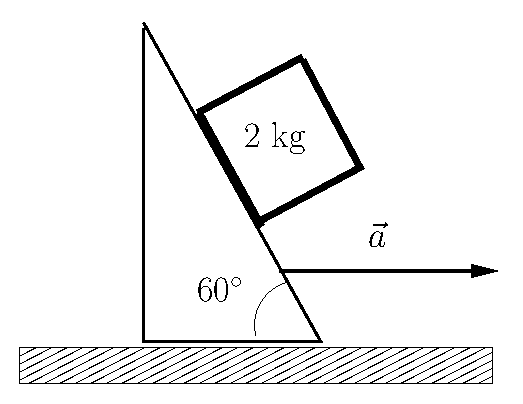
\includegraphics[width=2.5in]{additional_problems/wedge.eps}
    \end{center}
    \caption{Figure for Problem A\ref{prob:wedge}.}
    \label{fig:wedge}
  \end{figure}
  \begin{enumerate}
  \item What acceleration is required for this to occur?
  \item What would happen if the wedge were given an even greater
    acceleration?
  \end{enumerate}
  \label{prob:wedge}
\end{aproblem}


\begin{aproblem}{Using Forces to Predict Motion:  Dropping a Spring.}
  \begin{enumerate}
  \item Dangle your ``magic spring,'' holding it by one end, with the
    other end stretched out and hanging (relatively motionless) an
    inch or two above your other hand.  {\bf Don't do anything yet.}
    Think about what will happen when you let go of the top of the
    spring.

  \item {\em Before doing the experiment}, predict the order of the
    following five events.  Write down your prediction:. ({\it i}) The top
    end starts to move downward; ({\it ii}) The bottom end starts to move
    downward; ({\it iii}) The spring contracts halfway back to its
    unstretched size; ({\it iv}) The spring contracts all the way back to
    its unstretched size; ({\it v}) The bottom of the slinky hits your other
    hand.

  \item Now, once you have made your prediction, let go of the spring
    and see what actually happens.  You might have to do this a few
    times to figure out what the correct order is, or have a friend or
    two watch with you.  Write down the order of events as you
    actually observed them.

  \item Explain the results.  In doing so, you might want to draw a
    force diagram for the forces acting on the bottom loop of the
    spring both before and after the top of the spring is released.
    (Treat the bottom loop as a small mass hanging from the rest of
    the spring.)
  \end{enumerate}
\end{aproblem}

%\newpage

\begin{aproblem}{Force and Acceleration: Unwinding Yo-Yo.}
  \begin{enumerate}
  \item Wind up your yo-yo, and hold the end of the string (or put
    your finger through the loop).  Now, let the yo-yo fall out of
    your hand and unroll and drop downward (while holding the end of
    the string motionless).  Observe what happens.  Write down your
    observations.

  \item What can you say about the tension in the string while the
    yo-yo is unwinding?  Is the tension ({\it i}) equal to the weight of the
    yo-yo; ({\it ii}) less than the weight of the yo-yo but nonzero; 
    or ({\it iii}) zero?

  \item {\bf Explain} how you arrived at your answer.  You should be
    able to use the results of your observations, a force diagram and
    a simple use of Newton's 2$^{\rm nd}$ law to give a clear,
    definitive answer to the question. (We'll revisit this example
    again when we study rotations later in the semester.)

  \end{enumerate}
\label{prob:yoyoI}
\end{aproblem}


\begin{aproblem}{Circular Motion:  Around the World with Your Yo-Yo.}
  \begin{enumerate}
  \item Let the yo-yo hang at the end of the string and (holding the
    other end of the string) twirl it in a vertical circle so that it
    goes all the way around, being careful not to hit yourself or
    anyone around you in the head!  You should realize that you have
    to swing the yo-yo sufficiently fast; otherwise, it won't get all
    the way around.  Now, watch the string of the yo-yo as you swing
    it successively slower and slower until it falls out of the loop.

  \item Determine an expression for the theoretical minimum speed for
    the yo-yo at the top of its motion for it to complete the loop.
    Assume the string has a length $l$ and the yo-yo has a mass $m$
    and determine the minimum speed $v_{\rm top}$ as a function of
    $l$, $m$, and any fundamental constants.  \vspace{0.1in}

    {\bf Hints:} what happens to the string when the yo-yo is going
    just slightly too slow to be able to complete the loop?  What does
    this imply?  (The answer to this question is the key to solving
    this problem.)  Think back to Problem~A\ref{prob:return_ball}.
  \end{enumerate}
\end{aproblem}



%\parbox{4.6in}{
%\item {\bf Rough Ramp.}  Redo Tipler Chapter 4, problem 96, parts (a)
%and (b), but this time with friction.  Assume that the coefficient of
%kinetic friction between the $270\units{g}$ mass and the ramp is 
%$\mu_k = 0.1$.
%}

\begin{aproblem}{Friction Acting on Blow Dart.}
  \begin{enumerate}
  \item The goal of this exercise is to determine the average friction
    force acting on a blow dart as it slides across the floor.  Find a
    long, smooth, carpetless floor where you can fire a blow dart and
    watch it slide across the floor and eventually stop.  Smooth
    floors are the easiest surfaces to work with (the floors in Olin
    Science work well); for most other surfaces (e.g., carpeted
    floors), the dart will tend to bounce rather than slide.  You also
    might want to crouch down low and fire at a small, glancing angle.

  \item Determine the average friction force acting on the blow dart
    as it slows to a stop.  Make whatever measurements you deem
    relevant, and use the work-kinetic energy theorem --- this
    exercise is a snap if you do it this way, and a major pain if you
    try it any other way.  You can use your previous measurements of
    the initial speed of the blow dart once fired, and you might also
    be interested to know that the blow darts have a mass of $2.5\,
    \mbox{g}$ and a length of $6\units{cm}$, contain roughly
    $1.5\times 10^{24}$ protons and neutrons, and stick nicely to the
    front of your glasses.
  \end{enumerate}
\end{aproblem}



\begin{aproblem}{Blow Dart Survivor.}
  \begin{enumerate}
  \item Let's say that you were stranded on a deserted island and a
    few dozen {\em Federal Express} boxes washed ashore.  Let's say
    further that one of the boxes contained a {\em Bandito Blow Gun}.
    In addition to being delighted at being able to complete your
    PHYS~211 homework, you also realized that you could replace the
    suction cups with pointed tips and use this to hunt the birds that
    flew overhead.  Based on the measurements that you have already
    made, how low would a bird have to fly for you to have any chance
    of hitting it?

  \item To test this prediction, fire a dart straight up into the air,
    just look at its path, and see if your result seems reasonable.
    You might even try firing it up near a tree or building whose
    height you know approximately.
 
  \end{enumerate}
\end{aproblem}

\begin{aproblem}{Losing Mechanical Energy: Superballs.}
  \begin{enumerate}
  \item Take one of your superballs and release it from rest above a
    hard surface such as your desk or uncarpeted floor.  {\bf
      Questions:} Does it bounce back up to the height you released it
    from?  Is its mechanical energy conserved?

  \item Estimate how much mechanical energy is lost in one bounce of
    the superball.  Make whatever measurements you deem relevant, and
    explain your process.  Some information that you may find helpful:
    the small and large superballs have masses 8.5 and $25\,
    \mbox{g}$, respectively.

%     \item  Now, repeat with your Glow-in-the-Dark Squishy Eyeball.
%     Where do you think the mechanical energy of the Eyeball has gone?
%     To enhance some effects (and to gross you out a little bit), try
%     throwing the Eyeball against the floor, a wall, or a window.
%     What are some of the forms of energy where the mechanical energy
%     of the superballs or the eyeball may have gone?
  \end{enumerate}
\end{aproblem}



\begin{aproblem}{Spring Forward. } 
  A woman of mass $m$ rides upward on a spring-loaded ejector pad of
  spring constant $k$.  It moves upward from rest through a distance
  $x_0$ at which point the spring potential energy is zero.  Right
  then the woman leaves the spring with speed $v$ and flies upward
  reaching a maximum height $h$ above her starting position.
  \begin{enumerate}
  \item Make a sketch showing her starting position, launch point, and
    maximum height.

  \item Write down an energy expression for each position.

  \item Equate these expressions to determine the woman's ejection
    speed and maximum height above her initial position in terms of
    $k$, $x_0$, and $m$.
  \end{enumerate}
  \label{prob:spring_forward}
\end{aproblem}


\begin{aproblem}{Extreme Skiing.}
  Picabo Street has been challenged to test out a new ski event.  A
  loop of radius $R$ has been installed at the end of a ramp of height
  $h$ as shown in Fig.~\ref{fig:skiing}.  Assuming that the skier
  starts essentially from rest at the top of the ramp and ignoring
  friction, think about some of the forces the skier will have to
  withstand.  You will need to use both force and energy methods in
  this problem.
  \begin{figure}[h]
    \begin{center}
    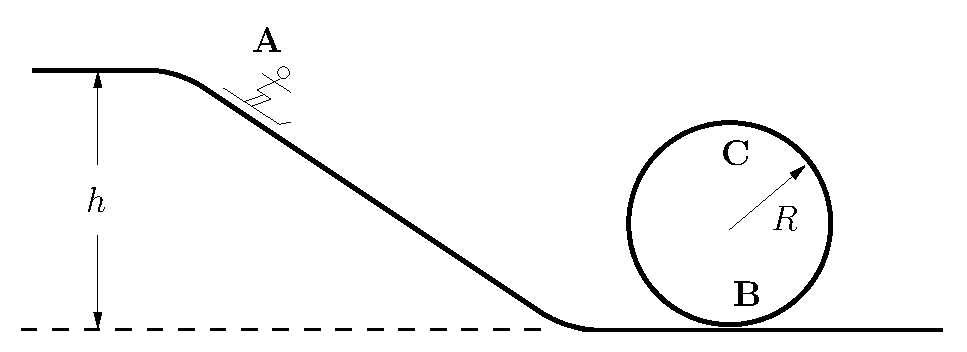
\includegraphics[width=4in]{additional_problems/skiing.eps}
    \end{center}
    \caption{Figure for Problem~A\ref{prob:skiing}.}
    \label{fig:skiing}
  \end{figure}

  \begin{enumerate}
  \item Picabo's legs have to provide support against the normal force
    of the ground on her legs.  Where along the ramp and the loop do
    her legs have to provide the maximum support?

  \item Determine the height $h$ in terms of the radius $R$ if the
    maximum force on her legs is to be 4 times her weight.

  \item With the height $h$ found in part (b), determine if she will
    be able to make it completely around the loop.

  \item Determine the minimum height $h$ in terms of the radius $R$
    such that Picabo can make it around the loop.  What is the maximum
    force on her legs for this height, in terms of her weight?
  \end{enumerate}
  \label{prob:skiing}
\end{aproblem}


\begin{aproblem}{Trapped in Space.}  
  A spacecraft drifting through the center of a giant cosmic dust
  cloud experiences a potential energy that varies with position as
  shown in Fig.~\ref{fig:trapped} ($d$ is the distance from the center
  of the dust cloud).  The spacecraft has a total mechanical energy of
  $E = -4\units{kJ}$.
  \begin{figure}[h]
    \begin{center}
    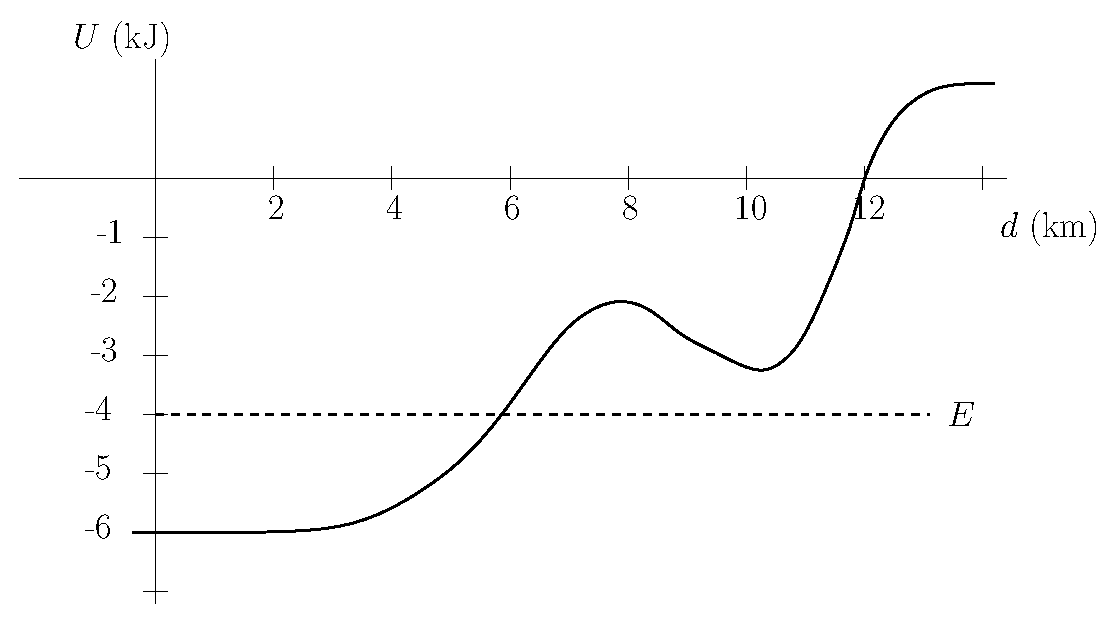
\includegraphics[width=4.5in]{additional_problems/trapped.eps}
    \end{center}
    \caption{Figure for Problem~A\ref{prob:trapped}.}
    \label{fig:trapped}
  \end{figure}
  \begin{enumerate}
  \item With this energy, what is the farthest distance the spacecraft
    could drift from the cloud's center?

  \item Determine the kinetic energy of the craft when it is $2\,
    \mbox{km}$ from the cloud center.

  \item Describe the motion of the spacecraft if the energy were
    $-2.5\units{kJ}$.
  \end{enumerate}
  \label{prob:trapped}
\end{aproblem}

\begin{aproblem}{Hopping Popper.}
  \begin{enumerate}
  \item In your kit, there should be a small rubber hemisphere that is
    referred to as a ``popper.''  If you turn it inside out and flex
    it for a few seconds, you can lay it on a table before it pops
    back into its original shape.  When it pops, it will jump up off
    the table, giving a nice demonstration of the conversion of
    potential energy into kinetic energy.

  \item Using whatever means you see fit, estimate the potential
    energy (in J) stored in the popper just before it pops.  (There's
    a really easy way to do this.)  The diameter of the popper is
    1~inch, its mass is $1.8\units{g}$, the hole in the center has a
    diameter of $2\units{mm}$, and there are approximately 3300
    students at Bucknell.
  \end{enumerate}
\end{aproblem}


\begin{aproblem}{Spring Slide Stop.}
  You push a block against a horizontal spring, compressing the spring
  by $15\units{cm}$.  When you release the block, the spring propels
  it across a level tabletop.  The block stops $75\units{cm}$ from
  its release point.  The spring constant is $200\units{N/m}$.
  Determine the magnitude of the friction force (assumed constant)
  that acts between the block and the table.
\end{aproblem}



\begin{aproblem}{Superball Stack!}
  Take your larger superball and carefully balance your smaller
  superball on top of it.  Release both from rest, and allow them to
  fall perfectly vertically in a line.  The large superball should hit
  the ground first and then collide (going up) with the small
  superball (still on its way down).  This requires lots of patience
  and luck, but if you get it, the result is incredible!  This can be
  understood by treating the various collisions as perfectly elastic
  collisions, which they almost are.  
  %If you can manage to do this with
  %all three superballs, you are in for a real treat!
\end{aproblem}



\begin{aproblem}{Blow Darts and Superballs.}
  There is nothing that makes a day more complete than firing a blow
  dart at a small, defenseless superball.  Before doing this, though,
  here is some relevant information: the blow dart has a mass of
  $2.5\units{g}$ and the small and large superballs have masses 8.5
  and $25\units{g}$, respectively.
  \begin{enumerate}
  \item Now, put your larger superball (the bug or skull ball) at the
    edge of a table and softly fire a blow dart directly at it (do it
    until the blow dart hits almost straight on).  By ``softly'' we
    mean don't blow as hard as you usually do.  If you do this
    correctly, the dart should bounce straight back, and the large
    ball will move forward with only a very small speed.

  \item Now, the main question: What changes do you have to make such
    that the blow dart will continue forward after a head-on collision
    with another object?  Predict what you need to do, write down your
    prediction, and then test out your theory.
  \end{enumerate}
  \label{prob:blow_dart_superball}
\end{aproblem}

\begin{aproblem}{Hogwarts Hijinks.}
  Harry and Hermione are playing in the GraviFree Room at Hogwarts.
  Harry (mass $55\units{kg}$) is floating motionless in the center
  of the room.  Hermione (mass $45\units{kg}$) pushes off from the
  wall and approaches Harry at a speed of $6.0\units{m/s}$.  Neglect
  air resistance in this problem.
  \begin{enumerate}
  \item As Hermione moves past Harry, he reaches out and grabs her
    outstretched hand, holding on tightly.  Determine the speed with
    which Hermione and Harry move after they grab hold of each other.
 
  \item Harry and Hermione notice Ron giving them a funny look, so
    they let go of each other.  Determine the speed with which
    Hermione moves after they let go.

  \item Determine the speed with which Harry moves after they let go.
     
  \end{enumerate}
  \label{prob:hogwarts}
\end{aproblem}


\begin{aproblem}{Railing in the Rain.}
  An open railroad car of mass $2\times 10^4\units{kg}$ is rolling
  without friction along a level track at $5\units{m/s}$ when it
  starts to rain.  After the car has collected $2000\units{kg}$ of
  water, it stops raining.  Assume that the rain fell perfectly
  vertically.
  \begin{enumerate}
  \item What is the rail-car's speed after it stops raining?

  \item After the rain has stopped, a hole in the bottom of the
    rail-car is unplugged, and the rain water begins to leak out of
    the hole at a rate of $5\units{kg/s}$.  What is the speed of the
    rail-car after half the rain water has leaked out?

  \item What is the speed after all the rain water has leaked out?
  \end{enumerate}
\end{aproblem}


\begin{aproblem}{Relative Velocities (Classical).}  
  A typical person walks with a speed of about $2\units{m/s}$
  relative to the ground.  While you are walking between classes,
  watch other students who happen to be walking in the same and
  opposite direction as you, and answer the questions in the following
  parts.
  \begin{enumerate}
  \item Choose a student walking in the same direction as you with the
    same approximate speed.  Note how far away that person is from
    you.  Then, after the two of you have walked for a few seconds,
    note again how far that person is from you.  Has the distance
    between the two of you increased, decreased or stayed roughly the
    same?  Assuming that you are both walking at a speed of $2\,
    \mbox{m/s}$ relative to the ground, what does your previous answer
    imply about the speed of the other person as measured in your
    reference frame?

  \item Do the same thing for a student walking in the opposite
    direction as you.  Answer the same questions as in part a).

  \item If you happen to see someone running to class, but going in
    the same direction as you, ask yourself the same questions as in
    part a).
  \end{enumerate}
\end{aproblem}

\begin{aproblem}{Measuring the Length of a Moving Object, Take 1.}
  Measuring the length of an object that is at rest with respect to
  you is pretty easy: one method is to take a ruler of some kind, hold
  it up to the object, and note where each end of the object is with
  respect to the ruler.
  \begin{enumerate}
  \item What difficulties arise if you try to measure the length of an
    object that is moving with respect to you using the technique
    described above? 

  \item Other methods need to be developed to measure the length of a
    moving object.  We'll have you try an approach that employs a
    group of people.  [We will do the following as a class exercise
    during problem session, so you won't have to gather a group of
    your own.]  Go outside, and line up in a row, parallel to a street
    with some automobile traffic.  (Please stand a safe distance away
    from the street!).  Stand so that there is approximately equal
    distance between you and your nearest neighbors \medskip

  \item Your instructor will stand across the street.  When a car
    comes by, your instructor will yell ``Now!''.  If the front of the
    car is directly in front of you, {\bf raise your hand} and {\bf
      keep it raised}.  If the back of the car is directly in front of
    you, {\bf raise your hand} and {\bf keep it raised.}  (By yelling
    ``Now!'' your instructor has basically synchronized your clocks,
    so that you are making your measurements --- i.e., raising your
    hand --- simultaneously.  You'll see in Problem
    A\ref{prob:synchronizeA} that to make this measurement even more
    carefully, we would have to come up with a better method of
    synchronization.  We'll discuss some thorny issues involving
    simultaneity in an upcoming lecture.)  \medskip

  \item Now, measure the distance between people who have their hand
    raised.  How is this distance related to the length of the car?
    Does it matter how fast the car is going in using this technique?
  \end{enumerate}
  \label{prob:moving_objI}
\end{aproblem}

\begin{aproblem}{Measuring the Length of a Moving Object, Take 2.}
  In problem A\ref{prob:moving_objI} you measured the length of a
  moving object using several people and synchronization.  In this
  problem, you will develop a technique that you could use on your
  own.
  \begin{enumerate}
  \item Assume that you know the velocity of the car (say the car is
    going the speed limit), and that your available tools are a ruler
    and a clock.  Figure out a method to determine the length of the
    moving car.  Describe what you would do and what you would
    measure. and how you would use the results of your measurement to
    determine the length.

  \item You likely measured a time interval and/or a distance.  Think
    how the driver of the car views the situation, especially if the
    speed were relativistic (say if the car were going at $0.8c$
    relative to you).  Would the driver of the car agree with your
    measurement of the time interval and/or distance?  Would she think
    your measurements are too high?  too low?  correct?

  \end{enumerate}
\end{aproblem}

\begin{aproblem}{Synchronization, Simultaneity and Spacetime Diagrams.}
  \begin{enumerate}
  \item Grab a friend or roommate (it doesn't have to be someone
    taking PHYS 211).  Stand on opposite sides of a room or a long
    hallway (the larger the separation distance, the better).  Throw a
    ball to your friend (or have that person throw the ball to you).
    Draw a qualitative spacetime diagram of this situation, showing
    world lines for you, your friend, and the ball.

  \item Your next goal is to have both of you clap your hands at
    precisely the same time, but you have to keep your eyes closed
    while doing it.  Here's an approach that you might try: you could
    say (loudly), ``On the count of three, we'll both clap our hands.
    One, two, THREE!''  Go ahead and try this, and then comment on
    inaccuracies in this method (i.e., why doesn't this work?).  Draw
    a spacetime diagram to support the argument.

  \item See if you can figure out a way that will result in you and
    your friend clapping at the same time.  Write down the method, and
    draw a spacetime diagram that demonstrates that this is a good
    approach.
  \end{enumerate}
\label{prob:synchronizeA}
\end{aproblem}


\begin{aproblem}{Life in a Relativistic World, Part I.}
  A typical person walks with a speed of about $3\units{mph}$
  relative to the ground.  For this problem, imagine that the speed of
  light were actually $4\units{mph}$ rather than $3.0\times 10^8\units{m/s}$.

  Walk across campus, perhaps on your way to or from class or going to
  dinner.  Choose a time when there is a lot of activity around you
  (cars moving around, other people walking around, etc).  While you
  are walking, watch everything around you.  Note what you see, what
  you feel, whatever you experience (when you are moving, waiting to
  cross a street, etc.), and think about how any of these things would
  be different if the speed of light were $4\units{mph}$.  {\bf
    Write a couple of paragraphs summarizing your thoughts.}  And feel
  free to discuss this with other people in the class.  (Some things
  to think about in particular: length contraction, time dilation, and
  simultaneity --- all of these things would be {\em very} noticeable
  in this hypothetical scenario.)

  If you really think about a lot of the things around, you should
  come to the conclusion that if $c$ were really $4\units{mph}$, it
  would truly be a whacked-out, psychedelic,
  something-out-of-a-Salvador-Dali-painting experience.
  \label{prob:rel_worldI}
\end{aproblem}


\begin{aproblem}{The Real Potential of a Superball.}  
  Pick up your largest superball and just stare at it for a little
  while.  Does this look like it contains a lot of energy?  Now,
  estimate its mass (or alternately look back at the Problem
  A\ref{prob:blow_dart_superball} where the mass is given) and
  determine the rest energy of the superball (in Joules).  Now,
  consider that an atomic bomb releases $10^{14}$ to
  $10^{15}\units{J}$ of energy; consider also that a typical household
  uses about $10^{10}\units{J}$ of energy per year.  Stare at your
  little ball again.  Write a sentence or two about your thoughts.
  (Feel free to post your thoughts on the ``Questions'' page at the
  course web-site if you want to share them.)
\end{aproblem}

\begin{aproblem}{Life in a Relativistic World, Part II.}  
  Let's think a little more about what it would be like walking across
  campus if the speed of light were $4\units{mph}$ rather than
  $3\times 10^8\units{m/s}$.  You've already thought about time
  dilation, length contraction and simultaneity in problem
  A\ref{prob:rel_worldI}.  Now, think about what the relationship $E =
  mc^2/\sqrt{1-v^2/c^2}$ would mean in a relativistic world.
  \begin{enumerate}
  \item If the speed of light were $4\units{mph}$, how much {\em
      kinetic} energy would be involved in walking at a speed of
    $3.5\units{mph}$?  (Use your own body mass in these estimates.)
    How much kinetic energy would you have walking at $3.8\,
    \mbox{mph}$?  How do you think you would feel as you start trying
    to walk faster and faster, past $3.0\units{mph}$, past $3.5\,
    \mbox{mph}$, past $3.8\units{mph}$, past $3.9\units{mph}$,
    \dots ?

  \item What do you think might happen if you collided with another
    person if you were both walking with a speed of $3.8\units{mph}$
    but in opposite directions?
  \end{enumerate}
\end{aproblem}

\begin{aproblem}{Life in a Really Relativistic World.} 
  Common misconceptions about relativity abound.  You'll hear people
  say that relativity states that ``if you are on a ship traveling
  close to the speed of light, your mass increases to infinity, you
  shrink down to zero size, and you never age.''  Statements like this
  have led people to think that life would be very strange on such a
  spaceship.  We want you to experience what it really would be like
  to be on such a spaceship. 

  So, go ahead and do this experiment.  Hop on a spaceship that is
  traveling at a speed of at least $0.8c$ relative to some reference
  frame.  Before you start saying that we've completely cracked up,
  there is a spaceship that everyone in this class has access to that
  meets this requirement.  (Hint: the name of the ship starts with the
  letter $E$ and its name rhymes with {\em birth}, and it is currently
  traveling at a speeds of greater than $0.9c$ relative to distant
  galaxies and quasars.) 

  {\bf Question:} do you feel at all strange being on such a ship?
  Write a sentence or two of your thoughts about this.  (Feel free to
  post your thoughts on the ``Questions'' page at the course web-site
  if you want to share them.)
\end{aproblem}

\begin{aproblem}{Photon Absorption} 
  An elementary particle has a rest mass of \break $1125\units{MeV/$c^2$}$,
  and is motionless in some reference frame.  A photon with momentum
  $750\units{MeV/$c$}$ strikes the particle and is absorbed, leaving
  an ``excited'' particle that is recoiling and nothing else.
  Determine the mass and recoil velocity of the excited particle after
  the interaction.
  \label{prob:photon_absorption}
\end{aproblem}

\begin{aproblem}{Let There Be Light.}  
  Particle A of mass $400\units{MeV/$c^2$}$ collides with the
  stationary particle B of mass $350\units{MeV/$c^2$}$.  The result of
  this collision is a single particle C at rest, and a
  $300\units{MeV}$ photon.  Determine the mass of particle C.
  \label{prob:light}
\end{aproblem}


\begin{aproblem}{What's That Skull (or Bug) Doing in My Superball? }
  We can take advantage of the poor bugs and skulls trapped in your
  larger superball to comment on the rotation of the ball.
  \begin{enumerate}
  \item Take your superball and rotate it slowly, watching the object
    as it rotates.  You can either do this in your hand, or toss it
    gently with a little rotation --- whichever enables you to see the
    object spinning easiest.  Try rotating it quickly as well.  What
    can you say about the motion of the middle portion of the object,
    as opposed to the motion of the part of the object farthest from
    the middle?  How does your answer to the previous question relate
    to the equation $v = r\omega$ for tangential speed?

  \item Now, drop the superball straight down while spinning it very
    rapidly about a horizontal axis.  The best way to do this is to 
    use two hands to get it
    spinning as fast as you can while releasing the ball.  What
    happens when the ball bounces?  Specifically, does it bounce
    straight up?  Why not?  (You'll want to use a diagram and Newton's
    $2^{\rm nd}$ and $3^{\rm rd}$ laws to support your argument.)
    Also, what happens to the angular velocity of the superball after
    it bounces?  Explain {\em why} this happens.  (Consider the torque
    acting on the ball when it bounces on the floor.)

  \item (Optional) If you are good at spinning the ball, try this:
    toss the ball slightly away from you, but spinning with the top
    toward you.  If you do this well, you can get the ball to bounce
    back and forth on the ground.  Explain {\em why} this happens.

  \end{enumerate}
\end{aproblem}

\begin{aproblem}{Yo-yos (revisited) with Rotations.}
  We're going to repeat Problem A\ref{prob:yoyoI}, but this time we're
  going to be quantitative and take rotation into account.
  \begin{enumerate}
  \item Count how many turns of the string are required to wind up the
    yo-yo all the way.  From this, calculate $\Delta\theta$ for the
    yo-yo to unwind completely (in radians).  Now, holding the end of
    the string, let the yo-yo unwind all the way, and estimate the
    time for it to reach the bottom (within a couple of tenths of a
    second). Since the angular acceleration is constant during this
    process, you should be able to take two integrals of $\alpha$ to
    find that $\Delta\theta = \alpha t^2/2$.  From this information,
    determine the angular acceleration of the yo-yo as it falls.

  \item Now estimate the average radius of the spool (i.e., the
    average distance of the point-of-contact of the string from the
    center of the yo-yo), and use this information to estimate the
    linear acceleration of the yo-yo during its fall.  Then, use this
    information (along with a force diagram and Newton's second law)
    to determine the tension in the string while the yo-yo is falling.
    Note: the mass of the yo-yo is $52\units{g}$, its total
    thickness is $3.5\units{cm}$, and it fits nicely in your pocket.

  \item Is your result from part (b) for the tension consistent with
    the qualitative answer from Problem~ A\ref{prob:yoyoI}?

  \end{enumerate}
\end{aproblem}

\begin{aproblem}{As the Ball Turns.}
  A solid $1.4\units{kg}$ ball with diameter $15\units{cm}$
  rotates about its diameter at 70 revolutions per minute.
  \begin{enumerate}
  \item Determine the kinetic energy of the solid ball.
  \item If the ball had the same mass and diameter, but all the mass
    was at the outer surface of the ball (in other words, the ball
    were hollow), would the ball have more or less kinetic energy than
    you calculated in part a)?  Assume this hollow ball has the same
    angular speed.
  \item Back to the solid ball again.  If you add an additional $2\,
    \mbox{J}$ of rotational kinetic energy, determine the solid ball's
    new angular speed.
  \end{enumerate}
  \label{prob:ball_turns}
\end{aproblem}

\begin{aproblem}{Yo-yos, mechanical energy, and angular momentum.}
  \begin{enumerate}
  \item Unwind the yo-yo and rotate it in a vertical circle at the end
    of its string.  Once it is going, allow the yo-yo string to wrap
    around your arm --- the result should be that the yo-yo spirals
    inward until all the string is wrapped around your arm.  Do this a
    few times and watch the yo-yo as it spirals inward.  Do you think
    the yo-yo is speeding up, slowing down, or going at basically the
    same speed during this process?  (Watch the yo-yo very carefully
    here --- your eyes can easily trick you.)

  \item Now, think about this process both from a perspective of
    mechanical energy and angular momentum.  Which of these quantities
    do you think are conserved during this process (or do you think
    that neither or both are conserved)?  Justify your answers: for
    angular momentum, you'll need to show either that torque acting on
    the yo-yo is zero or non-zero, and for energy, you'll need to
    explain either that work is or is not being done on the yo-yo.
    Based on these answers, should the yo-yo be speeding up, slowing
    down or basically going at the same speed while spiraling inward?

  \item Now do the same thing again, but this time, instead of letting
    the string wind around your arm, thread the string through a PVC
    tube (which we'll provide in problem session) and pull the string
    through the tube to pull the yo-yo inward.  Answer all the same
    questions that you did in parts a) and b).
  \end{enumerate}
\end{aproblem}

\newpage
\begin{aproblem}{Yo-yos and torque.}
  \begin{enumerate}
  \item Take a partially-wound (i.e., partially-unwound) yo-yo and
    place it on a level surface such that it could roll if pushed or
    pulled.  Now, predict which way it will roll if you pull the
    string straight up.  (Justify your prediction with diagrams and by
    considering the torque around the point of contact between the
    yo-yo and surface.)  Try the experiment --- were you correct?  If
    not, justify what actually happened.

  \item Now, do this again, but this time let the string go over the
    top of the yo-yo and pull it parallel to the table.  Again, first
    make a prediction about which direction the yo-yo will move (and
    justify it), then try the experiment.  Again, if you were not
    correct in your prediction, justify what actually happened with
    diagrams and Newton's laws.

  \item Finally, predict which way the yo-yo will move if the string
    goes underneath the yo-yo, and you pull it parallel to the table.
    (Again, justify your prediction with a diagram and by considering
    torque about the point of contact.)  Try the experiment.  Were you
    correct?  Again, if you were not, then justify what you actually
    saw.
  \end{enumerate}
\end{aproblem}

\begin{aproblem}{When Wheels Collide.}  
  Two solid wheels of identical mass but different radii ($R$ and
  $2R$) are spinning on the same axle (on very smooth bearings).  The
  wheels are spinning in opposite directions, but with the same
  angular speed $\omega_i$, as shown in Fig.~\ref{fig:wheels}.  The
  two wheels are slowly brought together, and the resulting frictional
  interaction between the touching surfaces eventually brings the
  wheels to a common angular speed $\omega_f$.
  \begin{figure}[h]
    \begin{center}
    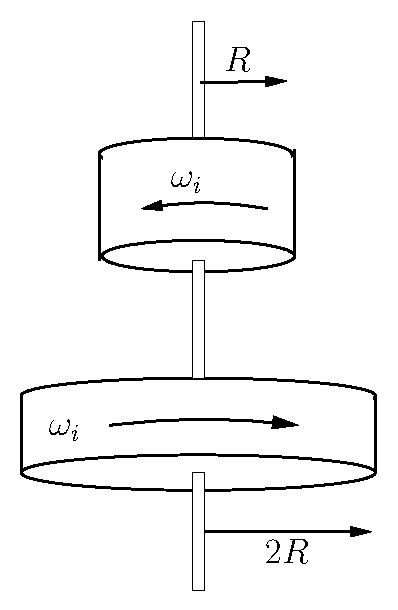
\includegraphics[width=1.5in]{additional_problems/wheels.eps}
    \end{center}
    \caption{Figure for Problem A\ref{prob:wheels}.}
    \label{fig:wheels}
  \end{figure}
  \begin{enumerate}
  \item Determine $\omega_f$ in terms of $\omega_i$.
  \item Are the wheels now rotating in the original rotation direction
    of the larger or the smaller wheel?
  \end{enumerate}
  \label{prob:wheels}
\end{aproblem}



\begin{aproblem}{How much do you suck?}
  \begin{enumerate}
  \item In problem session, you will be provided with a container that
    can hold water and a piece of flexible tubing.  Fill the container
    with some water and place the container on the floor.  Take your
    piece of flexible tubing and put one end into the water and stand
    up with the other end.  Put the other end into your mouth and
    breath in, pulling the water up the tube.  Don't breath in the
    water --- that wouldn't be very fun. (That shouldn't be a problem
    because if you are standing up, you won't be able to get the water
    all the way up the tube anyway.)  Estimate the maximum height
    above the water surface that you can hold the water by continually
    breathing inward.  {\bf Important:} don't use your cheeks to suck
    on the tube.

  \item Now, use this height to determine the ``gauge pressure'' of
    your lungs when you suck (the difference between your lungs'
    pressure and atmospheric pressure).  To do this, determine the
    force required to hold up a column of water with height $h$ in a
    tube with cross-sectional area $A$ (keep things in variables ---
    don't put the numbers in yet).  Once you have the force, you
    should be able to get the gauge pressure ($\Delta p$) from the
    relation between force, pressure and area.  Then, put the numbers
    in.  What is the {\em absolute} pressure that your lungs achieve
    when you suck?

  \item If you could make a perfect vacuum with your lungs, what would
    be the maximum height that you could suck water up in a straw?

  \item Now, let's see how hard you can blow.  Fill up the tubing
    about 2/3 to 3/4 of the way with water.  The easiest way to do
    this is to bend down low and suck water again. (Do you notice how
    much easier it is to suck up the water when it doesn't have to
    climb as high?).  A little before the water reaches your mouth,
    stop sucking and lift up the two ends of the tubing to make a
    ``U'' shape.  Now, blow into one end while raising the opposite
    end.  If you have a friend to help, that would be good --- he/she
    can continually raise the other end to make sure that you don't
    blow the water out of the tubing.  Estimate the maximum height
    (above your mouth) that you can hold the water, and use this
    information to estimate the gauge pressure and absolute pressure
    of your lungs when you are blowing.

    {\bf Note:} What you have just done is a technique that is used
    all the time in the medical industry to measure lung performance
    in patients.  This is particularly useful for patients with lung
    cancer or various breathing disorders --- this kind of test can
    quickly and easily determine how well the lungs are functioning.

  \item If you made a straw several hundred miles long, stuck one end
    into the ocean and stuck the other end out into the vacuum of
    space, would the straw suck up all of the ocean water into space?
    Why not?  (In fact, the water wouldn't rise up at all in the tube.
    Try to figure out why it wouldn't.)
  \end{enumerate}
  \label{prob:suck}
\end{aproblem}


\begin{aproblem}{Dunking Birds and the Ideal Gas Law.}
  \begin{enumerate}
  \item We're not actually going to use the dunking bird in its
    intended purpose here (don't worry --- that will come).  Instead,
    grab the Bird's butt in the palm of your hand and wrap your hand
    around it.  Presumably, if your hand is at normal body temperature
    (37$^\circ$~C), the fluid in the Bird will rise up toward the
    head, leaving a larger volume of gas than when you started.

  \item Estimate the volume of the gas in the Bird's butt before and
    after you warmed it up with your hand.  Actually, you really only
    need to approximate the ratio of the two volumes $V_{\rm
      after}/V_{\rm before}$.  Now, determine the ratio of the
    temperature of your hand to the temperature of the air; using the
    cool PHYS 211
    thermometer-keychain-and-attractive-clothing-accessory to measure
    the temperature inside your closed hand and of the air.  (What
    units are you using for temperature?)  Using the ideal gas law,
    determine if the change in the volume is consistent with the
    change in the temperature.  (Show all your work here.)

  \item What else do you think is going on inside the Bird?  We're not
    expecting a complete answer --- this is more of a set-up to help
    motivate the next class.  But you should be able to use the ideal
    gas law to make some statements about what else is going on inside
    the Bird.
  \end{enumerate}
  \label{prob:birdI}
\end{aproblem}

\begin{aproblem}{Pressure and Force.} 
  It is fairly straightforward to estimate the pressure inside a blow
  dart's suction cup when it is sticking to something.  First, we'll
  look at it qualitatively, then put some numbers in.
  \begin{enumerate}
  \item Wet the suction cup on one of your darts and press it onto a
    flat, smooth surface so that it sticks.  (It's best to have the
    dart wet, because this will keep air from leaking in around the
    suction cup.)  Pull on the dart and note how much force is
    necessary to pull the dart off the surface.  You don't have to be
    quantitative here; simply comment on how difficult it is to pull
    off.

  \item While you are pulling on the dart, what is causing the force
    that pulls (pushes) the dart {\em back onto the surface}?  Of
    course, this is due to the pressure difference between the inside
    and the outside of the suction cup, but what {\em physically} is
    causing the force?  (Refer to the kinetic theory of gases to
    answer this.)

  \item Now, let's do this semi-quantitatively.  If you stuck the dart
    to the underside of a smooth surface, you could hang about $1\,
    \mbox{kg}$ of mass from the dart without it coming off.  Based on
    this, you can determine the maximum force (in N) that the dart can
    withstand before coming off the surface.  And once you have the
    maximum weight that it can hold, use the definition of pressure
    (in terms of force and area) to estimate the pressure within the
    suction cup.  Note: the suction cup has a diameter of about $1.8\,
    \mbox{cm}$.  (You should estimate the pressure {\em difference}
    between the air and the inside of the cup first, then you can get
    the absolute pressure inside the cup.)

  \item If there were a perfect vacuum inside the suction cup, what
    would be the maximum weight that it could hold?
  \end{enumerate}
\end{aproblem}


\begin{aproblem}{Balloons and Bottles.}
  \begin{enumerate}

  \item Do the following experiment: Get a glass drink container ---
    one of those juice/cranberry bottles will work, but a
    taller/deeper glass drink container is better.  (You might be able
    to pluck something out of one of the recycling bins if needed.)
    You'll need to stretch a balloon across the opening of the jar, so
    try that out to make sure you can do it, then take the balloon
    off.  Then, boil a small amount of water (you can use a microwave
    if you want, but make sure that the water is really hot and
    steaming).  Pour a small amount of the boiling water into the jar
    (cover only the bottom cm or so).  If the water is hot enough,
    there should be a noticeable amount of steam coming out of it.
    Then, stretch the balloon over the mouth of the jar and then watch
    the system as things slowly cool down.

  \item Describe what happens, and explain {\em why} it happens.  In
    particular, comment on any condensation of the steam that you see
    on the inside of the container.  Is this condensation important as
    far as the behavior of the balloon is concerned?

  \end{enumerate}
\end{aproblem}


\begin{aproblem}{Using Phase Transitions to Cool a Drink.}  
  You'll need to do this at lunch or dinner, or somewhere that you
  have access to ice.
  \begin{enumerate}
  \item Get three glasses or cups.  Fill one glass (let's call it
    glass A) with a mixture of ice and water (plenty of ice), and fill
    the other two glasses each halfway full with room temperature
    water.  Let the ice/water mixture in glass A sit for a few
    minutes: this will ensure that both the ice and the water in the
    glass are at temperature 0$^\circ$~C.

    Next, you are going to take out a fair amount of $0^\circ$~C ice
    from glass A (a spoon is a convenient way to do this) and dump it
    into glass B, one of the half-filled room-temperature glasses.
    Then pour an equivalent amount of $0^\circ$~C water from glass A
    into glass C, the other half-filled glass.  The idea is to compare
    the cooling effects of $0^\circ$~C ice compared to $0^\circ$~C
    water.

    Before doing the experiment {\bf predict} whether glass B and
    glass C should be equally cooled, or if not, which will be cooler.
    Write down your prediction.

  \item Now, go ahead and do the {\bf experiment}.  Record the results
    in your notes.  Is the result what you expected?  Use heat flow
    arguments to {\bf explain} why you obtained this result.

  \end{enumerate}

%This experiment should begin to convince you that you can cool a drink
%much more with an ice cube at $0^\circ\units{C}$ than with an equal
%amount of $0^\circ\units{C}$ water.  The idea of using phase
%transitions in cooling applications is very widespread; in fact,
%commercial air conditioners depend on some sort of fluid (like freon)
%that vaporizes easily (i.e. changes phase) to absorb the heat from the
%object or area that is being cooled.  
\end{aproblem}


\begin{aproblem}{The Dunking Bird, revisited.} 
  In Problem A\ref{prob:birdI}, you should have found that the
  temperature change alone wasn't enough to cause the volume change
  and the resulting movement of the fluid up into the Bird's head ---
  there must have been a significant change in $N$, the number of gas
  molecules in the Bird.

  \begin{enumerate}
  \item Explain how $N$ is increasing in the Bird's butt when you heat
    it with your hand.  Explain also how $N$ decreases in the head
    when the head is cooled.  What about the fluid inside the Bird ---
    why do you think the Dunking Bird is filled with methylene
    chloride instead of simply dyed water?

  \item Now, how is the head of the Bird cooled during its normal
    dunking operation?  Does the water in the glass have to be cooler
    than the room temperature?  Try the following experiment: try
    using water in the glass that is measured to be the same as room
    temperature or better yet, heat up the water to be several degrees
    above room temperature, and dip the Bird's head in this warm
    water.  {\bf Question:} does the Bird still dunk?  (The result
    might surprise you.)  So, how {\em does} the Bird's head cool?

  \item A Dunking Bird with a wet head is comparable in many respects
    to a person who is sweating on a hot day.  Based on what you know
    about phase transitions (melting, vaporization, etc.), explain
    {\em why} it is necessary for a person to sweat on a hot day.  Why
    doesn't a person sweat as much on cooler days?
  \end{enumerate}
\end{aproblem}


\begin{aproblem}{ Energy Stored in a Balloon.}
  \begin{enumerate}
  \item When you blow up a balloon, you are clearly doing work on the
    balloon.  Alternatively, you can say that the gas in the expanding
    balloon is doing work.  And this work goes into potential energy.
    {\bf Question:} where is that energy ``stored''?

  \item In this problem, we're going to estimate that stored energy
    using $W = \int P\, dV$.  We'll use the approximation that the
    pressure is almost constant (we'll estimate an average pressure)
    so that $W= P\, \Delta V$.  And since the air outside the balloon
    is doing negative work on the balloon while it expands, and we
    want the {\em net} work done by the gas, you can use the gauge
    pressure to get the net work done by the air while the balloon
    expands.

    To estimate the gauge pressure, you need to attach the balloon to
    the end of your flexible hose with a rubber band, blow the balloon
    up half-way, then make sure to pinch off that end of the balloon.
    Now, get some water into the tube (still holding the balloon end
    pinched off), and then hold up the tube (in a U-shape, with the
    balloon at one end and the open end of the tube at the other).
    Finally, release the balloon such that the gauge pressure of the
    balloon pushes the water in the tube.

  \item Use this technique to estimate the average gauge pressure (see
    problem A\ref{prob:suck} for a refresher if you have forgotten),
    and estimate the change in volume when the balloon is fully
    inflated.  From this, you should be able to estimate the energy
    stored in the balloon.
  \end{enumerate}
\end{aproblem}



\begin{aproblem}{The Thermodynamics of Blow Darts.}  
  Let's think about what happens when you fire a blow dart.  We'll use
  the results from problem A\ref{prob:suck} (in which you determined
  the gauge pressure that your lungs can produce) to estimate the
  ideal maximum speed that you could achieve when firing a blow dart.

  \begin{enumerate}

  \item When you blow on the dart, the pressure $P_{\rm lung}$ from
    your lungs pushes the dart down the tube while atmospheric
    pressure $P_0$ pushes the dart the other way.  Draw a quick sketch
    of the dart, and draw arrows corresponding to the forces $F_{\rm
      lung}$ and $F_{\rm atm}$ on the dart.  Considering that the dart
    has a cross-sectional area $A$, what is the net force acting on
    the dart when you fire?  Re-write this result in terms of the
    gauge pressure for your lungs.

  \item Now, use the result from A\ref{prob:suck} and the fact that
    the dart has a diameter of about $1.8\units{cm}$ to estimate the
    net force acting on the dart when you blow.  Now, considering that
    the active part of the blow gun is about $50\units{cm}$ long,
    estimate the work done on the dart when firing.  (Note: you'd get
    the same result by using $W = P_{\rm gauge}\, \Delta V$.)
    Finally, use the work to predict the exit speed for the dart when
    you fire.

  \item The answer that you get here might differ significantly from
    what you measured in Problem~A\ref{prob:dartI}.  Why do you
    suppose these two results could be so different?  Do {\bf not} use
    ``human error'' anywhere in your response!
  \end{enumerate}
\end{aproblem}

\begin{aproblem}{Path Matters.} 
  One mole of an ideal monatomic gas is heated from $300\units{K}$
  to $600\units{K}$.
  \begin{enumerate}
  \item If the gas is held at constant volume, find the change in the
    gas's internal energy, the work done by the gas, and the heat
    added to the gas during this process.

  \item If the gas is held at constant pressure, find the change in
    the gas's internal energy, the work done by the gas, and the heat
    added to the gas during this process.
  \end{enumerate}
\end{aproblem}


\begin{aproblem}{Some Cycle.} 
  In the cycle shown below, $1.0$ mole of a
  monatomic ideal gas is initially at a pressure of $p_A=100\units{kPa}$
  and a temperature of $T_A=0^\circ\units{C}$.  The gas is heated at
  constant volume to $T_B = 150^\circ\units{C}$ and is then expanded
  adiabatically until its pressure is back to $p_C=100\units{kPa}$.
  Finally, the gas is compressed at constant pressure until it is back
  to its original state $A$.  Find

  \begin{enumerate}
  \item the temperature $T_C$ after the adiabatic expansion,
  \item the heat entering or leaving the system during each process,
  \item the efficiency of this cycle, and
  \item the efficiency of a Carnot cycle operating between the
    temperature extremes of this cycle.
  \end{enumerate}
  \begin{figure}[h]
    \begin{center}
      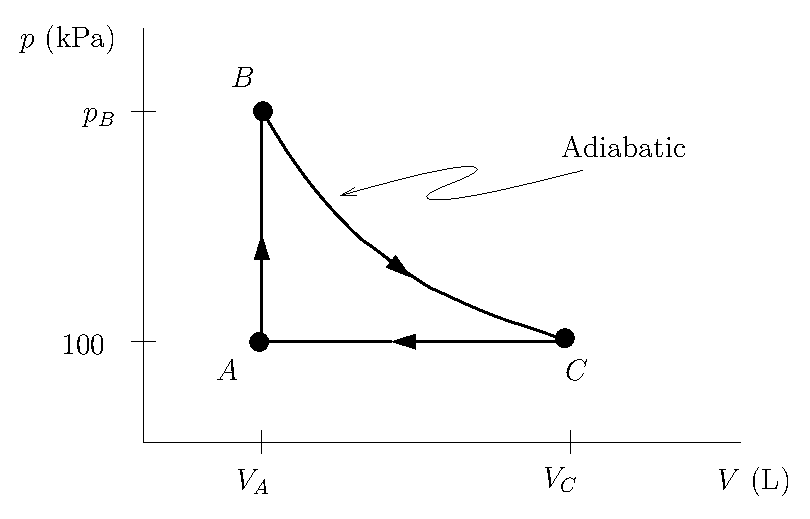
\includegraphics[width=4in]{additional_problems/cycle.eps}
    \end{center}
    \caption{Figure for Problem A\ref{prob:cycle}.}
    \label{fig:cycle}
  \end{figure}
  \label{prob:cycle}
\end{aproblem}



\begin{aproblem}{Dunking Birds as Heat Engines.} 
  First, get your Dunking Bird going.  You can actually operate it one
  of two different ways:
  \begin{itemize}
  \item[(I)] You can get the head wet and then just put it on a table.
    If the Bird is properly balanced (you may have to slide the metal
    piece up or down), then it should start going.

  \item[(II)] You could place the Bird on top of a TV or computer
    monitor and let the heat from that device warm the Bird's butt.
    ({\bf Warning:} Be careful if you do it this way: people have
    wound up with blue or red stained monitors and desks as well as
    having to clean up broken glass!)
  \end{itemize}


  \begin{enumerate}
  \item If the Dunking Bird is being powered by heating of its butt
    (i.e., Method II above), the gas/fluid in the butt will undergo
    several steps.  (The steps are actually continuous, but we'll
    break them up to make this easier to plot.)  ({\it i}) As the butt heats
    up, the pressure of the gas inside increases.  (Do you remember
    why?  It isn't just the change in temperature.) ({\it ii}) After the
    pressure has increased, the fluid is forced out of the butt, and
    the volume of gas in the butt increases.  ({\it iii}) The Bird tips over
    and the air in the butt and the air in the head are connected,
    causing a quick drop in the pressure of the gas in the butt down
    to its initial value.  ({\it iv}) The Bird stands up again, and the
    fluid runs down into the butt, decreasing the volume of gas in
    there.

    Plot the sequence described above on a $P$-$V$ diagram.  Do you
    have a cyclic process here?  Show the work for the engine cycle on
    your $P$-$V$ diagram.

  \item Repeat part (a), but for Method I (where the Bird's head is
    cooled by evaporation).

  \item What is the hot reservoir for this engine?  What is the cold
    reservoir?  What is the work done by the Bird (in words)?  Draw an
    engine diagram for the Bird.
 
  \end{enumerate}
\end{aproblem}


\begin{aproblem}{Entropy and the Second Law.}
   \begin{enumerate}
   \item Scatter at least 10 coins over a large surface area.  Then,
     carefully pick them all up and stack them into a neat pile.  Has
     the entropy of the coins increased, decreased or stayed the same?
     Use arguments based on probability to answer this question.
     (e.g., ``It is more probable that you'd \dots '').

   \item Is your answer consistent with the Second Law of
     Thermodynamics?  (The answer must, of course, be yes, but you
     might have to think a bit to figure out how to reconcile this
     with the Second Law.)  Explain your reasoning.
   \end{enumerate}
\end{aproblem}


\begin{aproblem}{Macrostates and Microstates.} 
  This problem gives you practice with the idea of macrostates vs.\
  microstates, in a different context than that provided in the
  reading.  Let's think about macrostates vs.\ microstates for the
  rolling of two six-sided dice. 
 
  When you roll two six-sided dice, each die can show a 1 through 6.
  The SUM of the numbers showing on the two dice is an integer from 2
  through 12.  That SUM is the macrostate.  The microstate is the
  specific combination that resulted in that macrostate.  So for
  example, if you rolled two six-sided dice, and the total of the two
  dice was an 8, that total could have been obtained a number of
  different ways: (2 and 6), or (3 and 5), etc.  In this example, the
  MACROSTATE is the sum 8, and some of the MICROSTATES associated with
  that macrostate are (2 and 6) or (3 and 5).

  \begin{enumerate}
  \item Consider all of the possible macrostates for this system of
    two six-sided dice.  For each macrostate, write down all the
    possible microstates associated with that macrostate.  Assume that
    the dice are distinguishable from each other, which means that
    there is a difference between (2 and 6) or (6 and 2).  Which
    macrostates have the most microstates associated with it/them?
    Which macrostates have the fewest microstates associated with
    it/them?  Use this to argue which macrostates are the most
    probable, and which macrostates are the least probable.

  \item Now, roll two six-sided dice 10 times, and record the
    macrostates that you observe. (If you don't have access to dice,
    you'll be able to do this part in problem session.)  Does your
    experimental evidence support your predictions from part (a); in
    other words, was the most probable macrostate clearly rolled more
    than the least probable macrostate?  You may be surprised by your
    results.  What do you think you need to do in order for the
    predictions to more accurately model the results of the
    experiment?  We'll collect data from the entire class for the
    number of times your most probable macrostate came up, and the
    number of times your least probable macrostate came up.

  \end{enumerate}
\end{aproblem}



\begin{aproblem}{Playing with the Period of Oscillation.}
  \begin{enumerate}
  \item Take your round metal spring, hold it by one end, and let the
    other end oscillate in the vertical direction.  Determine the
    period of oscillation using the following technique: find the
    approximate time for 5 complete periods and divide by 5.  Record
    the period of oscillation for the round metal spring.  What is the
    angular frequency of the oscillator?

  \item Now, take your round metal spring and jam your return ball
    into one end of the spring (as you did in problem
    A\ref{prob:graphII}.)  (Note: you may want to increase the mass
    even more).  Hold the spring by one end, letting the end with the
    ball wedged in dangle freely so that it can oscillate in the
    vertical direction.  {\bf Predict} whether the period of
    oscillation will be {\em larger than}, {\em smaller than}, or {\em
      equal to} the period of oscillation you obtained in part (a).
    {\bf Justify} your prediction.  Try the {\bf experiment} --- were
    you correct?  If not, {\bf explain} what {\em actually} happened.

  \end{enumerate}
  \label{prob:period}
\end{aproblem}



\begin{aproblem}{Circular Motion Versus Oscillatory Motion.}
  \begin{enumerate}
  \item Have a partner hold one end of the round metal spring and
    rotate it so that the other end makes a horizontal circle.  Now,
    you should stand back a couple of meters, and with one eye closed,
    watch the rotating end of the spring from the side so that the
    motion appears as though it is on a line.  If you view it from an
    appropriate angle, the motion should look exactly the same as if
    your friend were simply oscillating the spring back and forth
    along a line.

  \item To develop this further, ask your friend to go ahead and swing
    the spring back and forth instead of in a circle.  If you have one
    eye closed and if you are looking at it from the best angle, from
    your vantage point, it will look the same as if it were going in a
    circle.  And to develop this even more, have your friend either
    rotate the spring in a circle or oscillate it back and forth while
    you try to figure out which kind of motion the spring is
    following.  Treat it as a challenge --- your friend should try to
    fool you into thinking it is straight line motion when it is
    actually going in a circle or vice-versa.
  \end{enumerate}

  The point of this experience is to help clarify the idea that
  oscillatory motion can be thought of as one component of circular
  motion.  This idea will be very important when we talk about waves
  and interference in PHYS~212.
\label{prob:circ_vs_osc}
\end{aproblem}




\begin{aproblem}{Resonance}
  \begin{enumerate}
  \item We're going to map out (approximately) a simple resonance
    curve for your round metal spring.  You may use just the round
    metal spring, or you may use the round metal spring with the
    return ball jammed in one end.  Just make sure you indicate what
    you are doing.  In part (b) you will hold the spring by one end
    and let the other end dangle, and then oscillate your wrist at
    varying frequencies.  Before doing this, draw a sketch of what you
    would expect a resonance curve (amplitude of response versus
    driving frequency) would look like for the spring, assuming very
    little damping.  Based on your results from problem
    A\ref{prob:period}, what would you expect the frequency to be for
    the peak of this curve?  Write that frequency down.

  \item Now, hold the spring by one end and let the other end dangle.
    Wait until any residual oscillations damp out, then oscillate your
    wrist very slightly (amplitude of only a cm or less) at a
    frequency significantly smaller than the one that you predicted
    for the peak of the curve.  (Write down in your notes an
    approximation of what that frequency is.)  Do this for a few
    periods of oscillation, and comment on how the motion of the
    bottom end of the spring relates to the motion of your hand during
    this procedure.

  \item Now, repeat this again for a frequency that is significantly
    higher than the predicted resonance frequency, and comment on the
    results.  Finally, repeat this again for a forcing frequency close
    to your predicted resonant frequency.  Comment on your
    observations.

  \item Overall, do you observe resonant behavior?  Explain how your
    observations are consistent with ideas that we have discussed
    about resonance.
  \end{enumerate}
\end{aproblem}


\begin{aproblem}{How attractive are you?}
  We often take Newton's Universal Law of Gravitation for granted, but
  it was far from obvious in Newton's era that every object attracted
  every other object in the universe.  Why, for instance, don't we
  feel a gravitational attraction every time we come near another
  person or near another object?

  \begin{enumerate}
  \item The experience part: get very close to another person or to
    some other object that is close to your mass.  (It doesn't have to
    be another person --- you can stand close to a wall for the
    experience part.)  Now, try to see if you can feel any
    gravitational attraction.  In particular, can you feel the
    attraction getting stronger as you get closer?  Briefly comment
    (no more than one or two sentences) on what you feel.

  \item Based on this experience, do you think Newton's law of
    gravitation is obvious?

  \item Now, let's put some numbers on this experience.  Estimate your
    mass and the mass of the other person or object, and estimate the
    smallest separation between the two of you (estimate the distance
    between the center of you and the center of the other
    person/object).  Throw these numbers into Newton's law of
    gravitation to come up with a numerical estimate of the
    gravitational attraction that you experienced.  Is this a force
    that is strong enough to be noticeable?  (You might want to
    compare this force with the weight of some objects.)

  \end{enumerate}
\end{aproblem}


\begin{aproblem}{Orbits in a Non-Keplerian Solar System, Part I.}
  Suppose that the gravitational force of attraction depended not on
  $1/r^2$, but rather was proportional to the distance between the two
  masses (like the force due to a stretched spring).  In a planetary
  system that felt this different form of gravity, what would be the
  relationship between the period of a planet and its orbital radius?
  Assume circular orbits.
  \label{prob:nonkeplerI}
\end{aproblem}


\begin{aproblem}{Orbits in a Non-Keplerian Solar System, Part II }
  This experience problem goes hand-in-hand with the previous problem,
  problem A\ref{prob:nonkeplerI}.  In that problem, you work out how
  the period of a planet's orbit depends on radius if the force of
  attraction grew linearly with distance, rather than dropping off as
  $1/r^2$.  It so happens that this is a very easy thing to test with
  your toy kit.

  \begin{enumerate}
  \item Take your round metal spring, hold it by one end, and twirl it
    slowly so that the other end makes a circle in a horizontal plane
    (similar to what you did in problem A\ref{prob:circ_vs_osc}).
    Determine the period of revolution using the following technique:
    find the time for 10 complete periods and divide by 10.  Now, do
    it again, but this time twirl it {\em really} fast so that it
    stretches out a lot, resulting in a circle of significantly larger
    radius.  Again, determine the period (time for 10 revolutions
    divided by 10).

  \item Do your results agree with your prediction from problem
    A\ref{prob:nonkeplerI}?  Specifically, when you increase the
    radius (by twirling faster), does the period grow linearly with
    radius, drop as $1/r$, remain the same, \dots ?

  \end{enumerate}
\end{aproblem}


\begin{aproblem}{Curved space.}
  \begin{enumerate}
  \item Blow up and tie off a balloon.  You are going to draw a circle
    on the balloon with a radius of $10\units{cm}$ as measured by a
    2-dimensional being that lived on this surface and wasn't aware
    that the surface was curved in a 3-dimensional world.  Mark a
    point on the balloon that will act as the center of the circle.
    Now, mark off a 10-cm portion of the string in your toy kit (or
    you can use your yo-yo string or dental floss).  Place one of end
    of that 10-cm segment at the marked point on the balloon and use
    the other end of the 10-cm segment like a drawing compass, pulling
    the string so that it is tight against the surface of the balloon
    and swinging it around in a circle, tracing out that circle on the
    balloon as you go.  The net result should be a reasonably clean
    circle with a 2-dimensional radius $r_{\rm 2D}$ (along the surface
    of the balloon) of $10\units{cm}$.

  \item Now, measure the circumference of the circle.  You can do this
    by taking the yo-yo string (or some other string) and wrapping it
    around the balloon until it lines up with the circle that you have
    just drawn.  Then, straighten out the string and measure its
    length.

  \item Is the circumference equal to $2\pi r_{\rm 2D}$?  Your result
    shouldn't bother you because you happen to live in a
    three-dimensional world, and you know therefore that the {\em
      real} center of the circle that you just drew is inside the
    balloon, so the {\em real} radius isn't $5\units{cm}$.  But if
    you couldn't comprehend a third dimension and lived on the surface
    of the sphere, would you find the result surprising?

  \item Now, imagine going outward a certain well-defined distance $R$
    from the center of our sun, and drawing a circle all the way
    around the sun with that distance as the radius.  Would you be
    surprised if the circumference of that circle were less than $2\pi
    R$?  (This is, in fact, what you would find if you could do this
    measurement without being burned up.)
  
  \end{enumerate}
\end{aproblem}

